\documentclass[a4paper]{article}
\usepackage{graphicx}
\usepackage{wrapfig}
\usepackage{caption}
\usepackage{subcaption}


\title{Selection Sort}
\author{Yarne Ramakers}
\date{\today}

\begin{document}

%\maketitle - had to comment as it took up too much space
\begin{center}
  Insertion Sort \\
  Yarne Ramakers \\
  \today \\
\end{center}

\begin{figure}[h]
  \begin{subfigure}[b]{0.5\textwidth}
    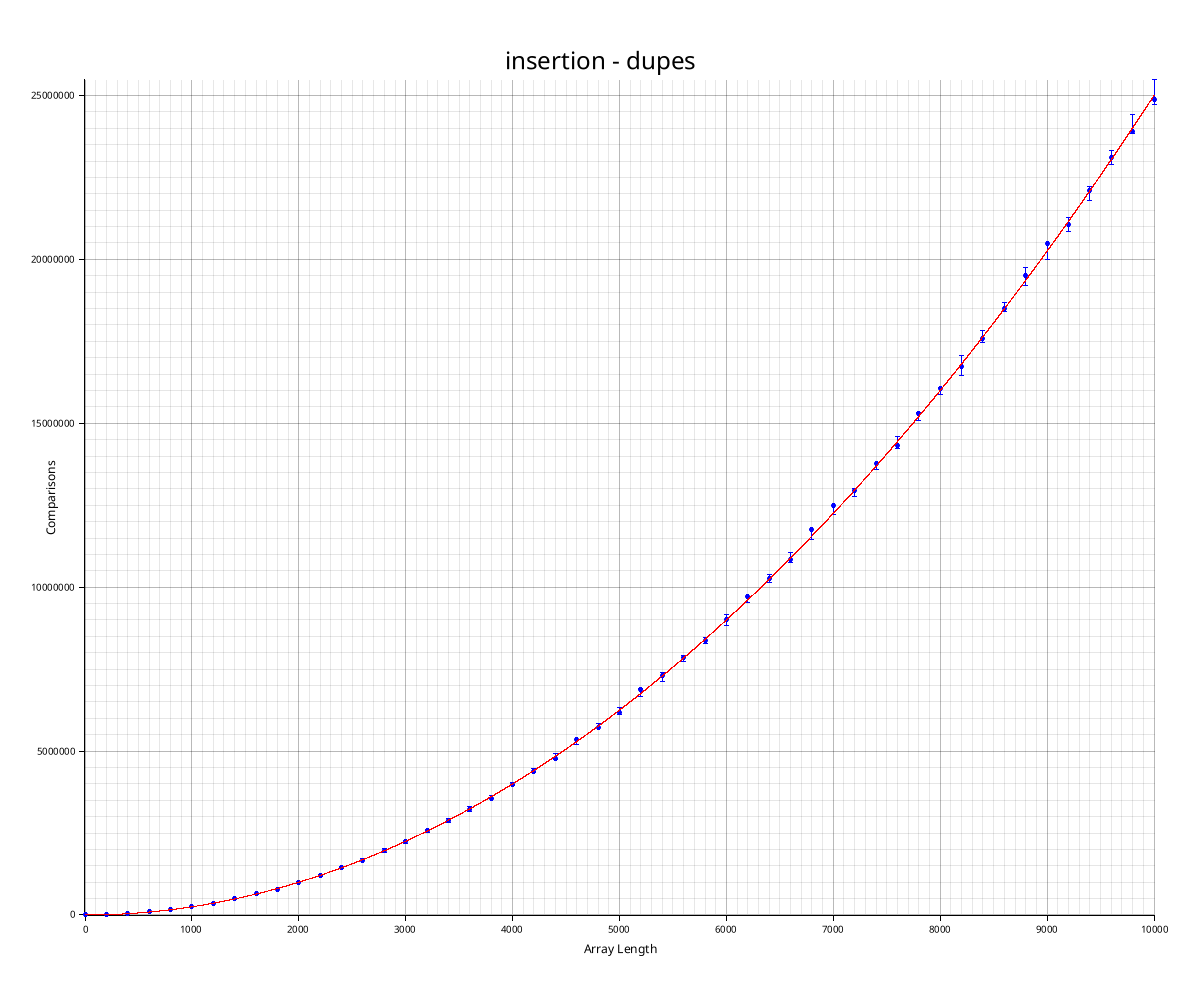
\includegraphics[width=\textwidth]{../plots/insertion-dupes.png}
    \caption{1/10th Unique Values}
    \label{fig:insertion-dupes}
  \end{subfigure}
  \begin{subfigure}[b]{0.5\textwidth}
    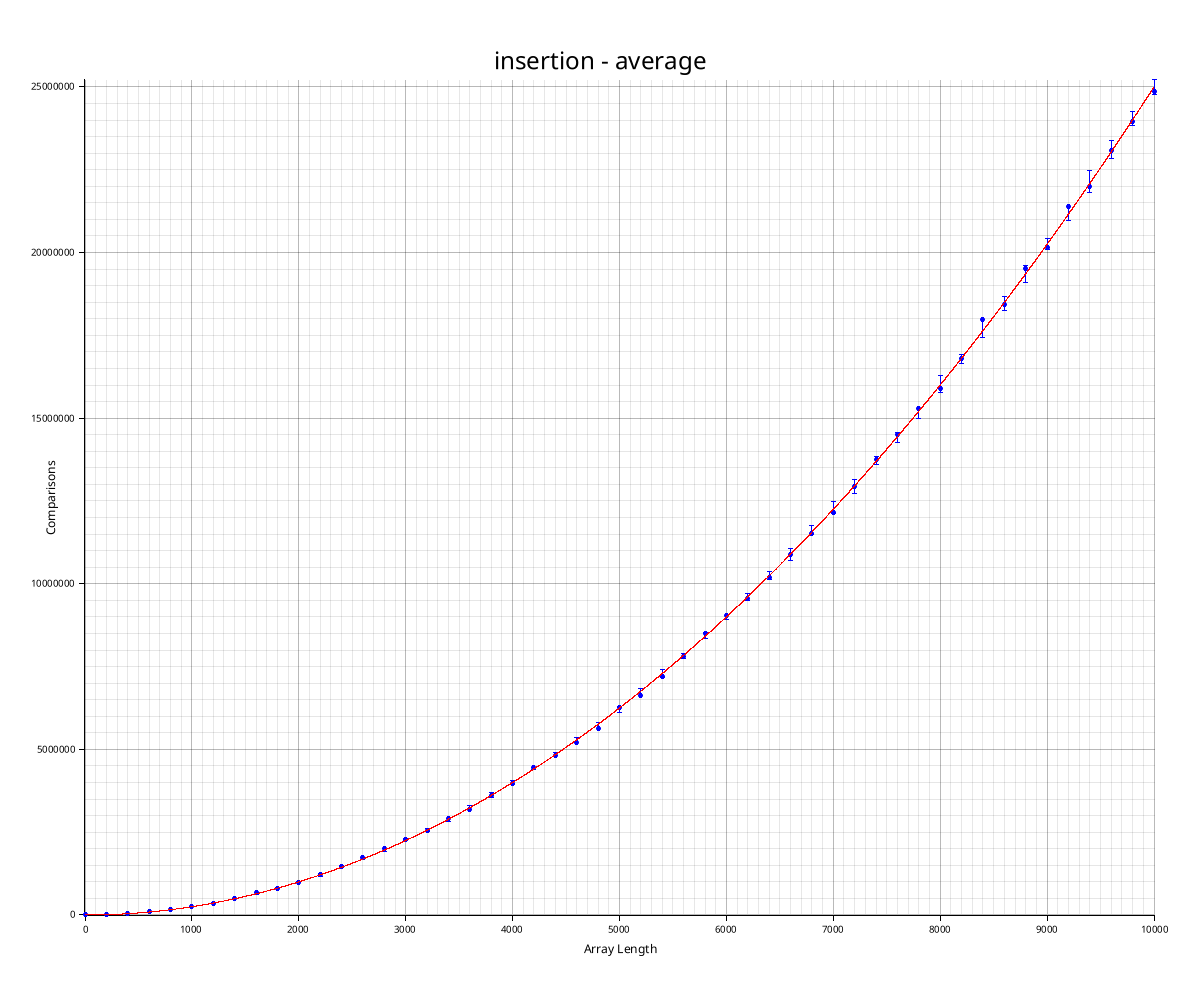
\includegraphics[width=\textwidth]{../plots/insertion-average.png}
    \caption{Average}
    \label{fig:insertion-avg}
  \end{subfigure}\hfill
\end{figure}

\section{Duplicate Values}
Insertion sort is getest op lijsten van lengte $n$ waarvan 1/5, 1/10, 1/20 en 1/40 van de waarden uniek zijn. 
In de grafiek \ref{fig:insertion-dupes} is de complexiteit van insertion sort te zien voor een lijst waarvan 1/10 van de waarden uniek zijn.
Met andere woorden elke waarde heeft nog 9 voorkomens in de lijst.
\par 
We merken op dat de complexiteit van insertion sort voor lijsten met duplicaten hetzelfde is als voor lijsten met unieke waarden.
Dit komt omdat insertion sort elke waarde vergelijkt en de grootste bijhoudt en vervolgens vanachter plaatst.
Omdat het algoritme niet weet dat er duplicaten zijn zal het algoritme nog altijd door de hele lijst moeten gaan om de grootste waarde te vinden.
\par
Het algoritme is voor elke lengte $n$ 10 keer uitgevoerd op een willekeurige lijst zoals hierboven beschreven.
We merken wel op dat de spreiding van de metingen dichter bij de theoretische complexiteit ligt dan bij lijsten met unieke waarden \ref{fig:insertion-avg}.
Dit komt omdat de lijsten met duplicaten minder variatie hebben in de volgorde van de waarden.
Er is meer kans dat elke waarde al op zijn plaats staat, in dit geval zijn er dan minder vergelijkingen nodig.

\section{Nearly Sorted}
Ik ben in een eerdere inzending tot de conclusie gekomen dat voor een bijna gesorteerde lijst de tijdscomplexiteit van insertion sort $\sim dn$ is met $d$ gelijk aan
de gemiddeld aantal verplaatsingen nodig om een element op zijn plaats te zetten. Ik genereer eerst een gesorteerde lijst en deel deze op in "chunks" van een lengte $l$
die ik dan shuffle. Enkel voor $l=10$ kwam ik uit dat insertion sort $\sim dn$ zal zijn met $d=3$, het gemiddeld aantal verplaatsingen nodig.
Dinsdag kreeg ik een bericht van Yendric Van Roey, die een rare bevinding had gedaan. In zijn metingen bleek dat voor elke $l \ne 10$ het niet gelde dat insertion sort
zich volgens $\sim dn$ zal gedragen.
\par
Yendric genereert zijn lijsten op een andere manier. Hij neemt namelijk een element en verplaatst het met een random index binnen het interval $[-k,k]$ en houd bij
welke hij al verplaatst heeft, zodat dit niet nog eens verplaatst wordt. Eerst dachten we dat zijn implementatie verkeerd was. Maar toen ik mijn functie uitprobeerde
met een andere $l$ kwam ik op exact dezelfde bevinding uit. Insertion sort zal zich beter gedragen dan $\sim dn$. Bij een $l=100$ zouden we verwachten dat insertion sort
zich gedraagt volgens $\sim 33n$, aangezien er gemiddeld 33 verplaatsingen nodig zijn per element om op de juiste plaats te komen, 
uit metingen bleek namelijk dat het zich gedraagt als $\sim 25n$.
\par
We hebben veel gezocht en gespeculeerd hoe dit kon komen. We kwamen namelijk uit dat insertion sort zich zal ongeveer gedragen volgens $\sim \frac{3}{4}dn$ met $d$
het gemiddeld aantal verplaatsingen. Uiteindelijk vond Yendric de correcte formule en deze bleek ook te kloppen voor mijn implementatie.
De gevonden formule is $\frac{n}{l}\sum_{i=0}^{l-1}\sim_{x=0}^{l-i}\frac{x}{l-i}=\frac{1}{4}(l+3)n$. Vullen we hier $l=10$ in komen we uit op $\approx 3.25n$ wat
inderdaad - op een paar duizendste na - de gevonden factor is voor mijn programma. Sterker nog, deze formule klopt voor eender welke $l$.
\par
We kunnen dus concluderen dat insertion sort bij deels gesorteerde lijsten zich niet zal gedragen volgens $\sim dn$ maar volgens $\frac{1}{4}(l+3)n$ met $l$ in dit
geval de grootte van de deellijst die geshuffelt is. 
